% -*- coding: utf-8 -*-

\documentclass[12pt,xcolor={rgb}]{beamer}

\usetheme{dirichlet}

% remove these two lines to hide footlines in (sub)section pages
\setbeamertemplate{at begin section}[normal]
\setbeamertemplate{at begin subsection}[normal]

\usepackage{arev}

%%%%%%%%%------------------------------------------------------------------------
%%%% 日常所用宏包

%% 控制页边距
\usepackage[top=2cm, bottom=2cm, left=3.2cm, right=2.cm,includehead,includefoot]{geometry}

%% 控制项目列表
\usepackage{enumerate}

%% 多栏显示
\usepackage{multicol}

%% hyperref宏包,生成可定位点击的超链接,并且会生成pdf书签
\usepackage[%
    pdfstartview=FitH,%
    CJKbookmarks=true,%
    bookmarks=true,%
    bookmarksnumbered=true,%
    bookmarksopen=true,%
    colorlinks=true,%
    citecolor=blue,%
    linkcolor=blue,%
    anchorcolor=green,%
    urlcolor=blue%
]{hyperref}

%% 控制标题
\usepackage{titlesec}

%% 控制表格样式
\usepackage{booktabs}

%% 控制目录
\usepackage{titletoc}

%% 控制字体大小
\usepackage{type1cm}

%% 首行缩进,用\noindent取消某段缩进
\usepackage{indentfirst}

%% 支持彩色文本、底色、文本框等
\usepackage{color,xcolor}

%% AMS LaTeX宏包
\usepackage{amsmath}

%% 一些特殊符号
% \usepackage{bbding}

%% 支持引用
% \usepackage{cite}

%% LaTeX一些特殊符号宏包
% \usepackage{latexsym}

%% 数学公式中的黑斜体
% \usepackage{bm}

%% 调整公式字体大小:\mathsmaller, \mathlarger
% \usepackage{relsize}

%% 生成索引
% \makeindex

%%%% 基本插图方法
%% 图形宏包
\usepackage{graphicx}

%% 多个图形并排,参加lnotes.pdf
\usepackage{subfig}

% \begin{figure}[htbp]               %% 控制插图位置
%   \setlength{\abovecaptionskip}{0pt}
%   \setlength{\belowcaptionskip}{10pt}
                                     %% 控制图形和上下文的距离
%   \centering                       %% 使图形居中显示
%   \includegraphics[width=0.8\textwidth]{CTeXLive2008.jpg}
                                     %% 控制图形显示宽度为0.8\textwidth
%   \caption{CTeXLive2008安装过程} \label{fig:CTeXLive2008}
                                     %% 图形题目和交叉引用标签
% \end{figure}
%%%% 基本插图方法结束

%%%% pgf/tikz绘图宏包设置
\usepackage{pgf,tikz}
\usetikzlibrary{shapes,automata,snakes,backgrounds,arrows}
\usetikzlibrary{mindmap}
%% 可以直接在latex文档中使用graphviz/dot语言,
%% 也可以用dot2tex工具将dot文件转换成tex文件再include进来
%% \usepackage[shell,pgf,outputdir={docgraphs/}]{dot2texi}
%%%% pgf/tikz设置结束


%%%% fancyhdr设置页眉页脚
%% 页眉页脚宏包
\usepackage{fancyhdr}

%% 页眉页脚风格
\pagestyle{plain}

%% 有时会出现\headheight too small的warning
\setlength{\headheight}{15pt}

%% 清空当前页眉页脚的默认设置
%\fancyhf{}
%%%% fancyhdr设置结束


%%%% 设置listings宏包用来粘贴源代码
%% 方便粘贴源代码,部分代码高亮功能
\usepackage{listings}

%% 所要粘贴代码的编程语言
\lstloadlanguages{}

%% 设置listings宏包的一些全局样式
%% 参考http://hi.baidu.com/shawpinlee/blog/item/9ec431cbae28e41cbe09e6e4.html
\lstset{
showstringspaces=false,              %% 设定是否显示代码之间的空格符号
numbers=left,                        %% 在左边显示行号
numberstyle=\tiny,                   %% 设定行号字体的大小
basicstyle=\footnotesize,                    %% 设定字体大小\tiny, \small, \Large等等
keywordstyle=\color{blue!70}, commentstyle=\color{red!50!green!50!blue!50},
                                     %% 关键字高亮
frame=shadowbox,                     %% 给代码加框
rulesepcolor=\color{red!20!green!20!blue!20},
escapechar=`,                        %% 中文逃逸字符,用于中英混排
xleftmargin=2em,xrightmargin=2em, aboveskip=1em,
breaklines,                          %% 这条命令可以让LaTeX自动将长的代码行换行排版
extendedchars=false                  %% 这一条命令可以解决代码跨页时,章节标题,页眉等汉字不显示的问题
}
%%%% listings宏包设置结束


%%%% 附录设置
\usepackage[title,titletoc,header]{appendix}
%%%% 附录设置结束


%%%% 日常宏包设置结束
%%%%%%%%------------------------------------------------------------------------

%%%%%%%%------------------------------------------------------------------------
%%%% 英文字体设置结束
%% 这里可以加入自己的英文字体设置
%%%%%%%%------------------------------------------------------------------------

%%%%%%%%------------------------------------------------------------------------
%%%% 设置常用字体字号,与MS Word相对应

%% 一号, 1.4倍行距
\newcommand{\yihao}{\fontsize{26pt}{36pt}\selectfont}
%% 二号, 1.25倍行距
\newcommand{\erhao}{\fontsize{22pt}{28pt}\selectfont}
%% 小二, 单倍行距
\newcommand{\xiaoer}{\fontsize{18pt}{18pt}\selectfont}
%% 三号, 1.5倍行距
\newcommand{\sanhao}{\fontsize{16pt}{24pt}\selectfont}
%% 小三, 1.5倍行距
\newcommand{\xiaosan}{\fontsize{15pt}{22pt}\selectfont}
%% 四号, 1.5倍行距
\newcommand{\sihao}{\fontsize{14pt}{21pt}\selectfont}
%% 半四, 1.5倍行距
\newcommand{\bansi}{\fontsize{13pt}{19.5pt}\selectfont}
%% 小四, 1.5倍行距
\newcommand{\xiaosi}{\fontsize{12pt}{18pt}\selectfont}
%% 大五, 单倍行距
\newcommand{\dawu}{\fontsize{11pt}{11pt}\selectfont}
%% 五号, 单倍行距
\newcommand{\wuhao}{\fontsize{10.5pt}{10.5pt}\selectfont}
%%%%%%%%------------------------------------------------------------------------


%%%%%%%%------------------------------------------------------------------------
%%%% 一些个性设置

%% 设定页码方式,包括arabic、roman等方式
%% \pagenumbering{arabic}

%% 有时LaTeX无从断行,产生overfull的错误,这条命令降低LaTeX断行标准
%% \sloppy

%% 设定目录显示深度\tableofcontents
%% \setcounter{tocdepth}{2}
%% 设定\listoftables显示深度
%% \setcounter{lotdepth}{2}
%% 设定\listoffigures显示深度
%% \setcounter{lofdepth}{2}

%% 设定段间距
\setlength{\parskip}{0.3\baselineskip}

%% 设定行距
\linespread{1}

%% 中文破折号,据说来自清华模板
\newcommand{\pozhehao}{\kern0.3ex\rule[0.8ex]{2em}{0.1ex}\kern0.3ex}

%% 设定itemize环境item的符号
\renewcommand{\labelitemi}{$\bullet$}

%% 设定正文字体大小
% \renewcommand{\normalsize}{\sihao}

%%%% 个性设置结束
%%%%%%%%------------------------------------------------------------------------


%%%%%%%%------------------------------------------------------------------------
%%%% bibtex设置

%% 设定参考文献显示风格
\bibliographystyle{unsrt}

%%%% bibtex设置结束
%%%%%%%%------------------------------------------------------------------------

\usepackage{xeCJK}

\begin{document}

\title{}
\author{2017年2月20日}
\date{}

\begin{frame}[plain]

\begin{center}
{\LARGE  数控转台控制系统设计 }

\vspace{1.1cm}
 \makebox[5em][s]{课程名称}:~
\underline{ \makebox[3cm]{ 机电一体化技术 }}\\
\makebox[5em][s]{教师姓名}:~
\underline{ \makebox[3cm]{彭可}}\\
\makebox[5em][s]{研究生姓名}:~
\underline{ \makebox[3cm]{高星}}\\
\makebox[5em][s]{学号}:~
\underline{ \makebox[3cm]{201580180367}}\\ \makebox[5em][s]{专业方向}:~
\underline{ \makebox[3cm]{机械工程}}\\	

\end{center}

\end{frame}

\section{数控转台介绍}

\begin{frame}{数控转台}
数控转台主要用于加工中心、数控镗床和铣床,为加工中心和数控铣床提供了回转坐标,通过第四轴、第五轴驱动转台或分度头完成等分、不等分或连续的回转加工,完成复杂曲面加工,使机床原有的加工范围得以扩大。
\end{frame}

\begin{frame}{传统数控转台结构}
\begin{enumerate}
	\item 采用高精度蜗杆蜗轮等传动;
	\item 伺服系统的驱动方式;
	\item 转台静止时必须处于锁紧状态;
	\item 导轨面由大型滚动轴承支承;
	\item 回转转台设有零点。
\end{enumerate}

\end{frame}

\section{需求分析}

\begin{frame}{需求分析}
\begin{enumerate}
	\item 数控机床的发展;
	\item 国内的数控转台市场;
	\item 发展及前景;
\end{enumerate}
\end{frame}

\section{机械部分设计}

\subsection{传动方案的选择}

\begin{frame}{传动方案传动时应满足的要求}
合理的传动方案主要满足以下要求:
\begin{enumerate}
	\item 机械的功能要求:应满足转台的功率、转速和运动形式的要求。
	\item 工作条件的要求:例如工作环境、场地、工作制度等。
	\item 工作性能要求:保证工作可靠、传动效率高等。
	\item 结构工艺性要求;如结构简单、尺寸紧凑、使用维护便利、工艺性和经济合理等。
\end{enumerate}
\end{frame}

\begin{frame}{传动方案及其分析}
由图\ref{方案设计}所示,数控转台的传动方案有两种:方案一为一级和二级都是齿轮传动;方案二为一级齿轮传动,二级蜗杆传动。

\begin{figure}[htb]
	\begin{center}
		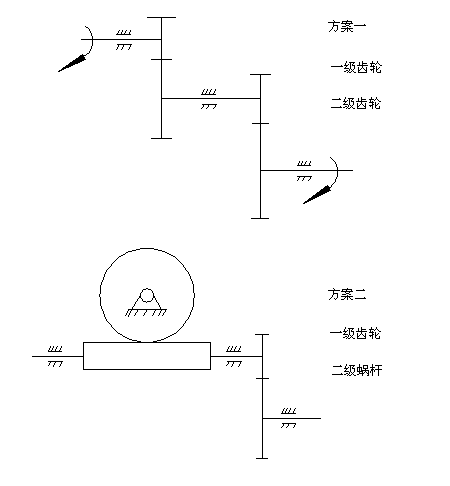
\includegraphics[width=5cm]{images/1}
		\caption{方案设计}  \label{方案设计}
	\end{center}
\end{figure}
\end{frame}

\begin{frame}{两种方案对比}
方案一的最大缺陷是:
\begin{enumerate}
	\item 总传动比小;
	\item 占用空间大;
	\item 只能使转台完成回转功能,无法使转台完成自锁。
\end{enumerate}
而方案二虽然传动效率低,但以上三个功能全部都能完成自锁。
所以数控转台传动方案为方案二:步进电机——齿轮传动——蜗杆传动——转台。
\end{frame}

\begin{frame}{蜗杆传动}
蜗杆传动有以下特点:
\begin{enumerate}
	\item 传动比大,在分度机构中可达1000以上。与其他传动形式相比,传动比相同时,机构尺寸小,因而结构紧凑。
	\item 传动平稳 蜗杆齿是连续的螺旋齿,与蜗轮的啮合是连续的,因此,传动平稳,噪声低。
	\item 可以自锁 当蜗杆的导程角小于齿轮间的当量摩擦角时,若蜗杆为主动件,机构将自锁。这种蜗杆传动常用于起重装置中。
	\item 效率低、制造成本较高  蜗杆传动方面:齿面上具有较大的滑动速度,摩擦磨损大,故效率约为0.7-0.8,具有自锁的蜗杆传动效率仅为0.4左右。为了提高减摩擦性和耐磨性,蜗轮通常采用价格较贵的有色金属制造。
\end{enumerate}
\end{frame}

\subsection{齿轮传动的设计}

\begin{frame}{选择齿轮传动的类型与材料}
\begin{enumerate}
	\item 选用直齿圆柱齿轮传动;
	\item 选用7级精度;
	\item 选择小齿轮材料为40Gr(调质),硬度为280HBS,大齿轮材料为45钢(调质);
	\item 选小齿轮齿数Z=24,大齿轮齿数取Z=72
\end{enumerate}
\end{frame}

\begin{frame}{按齿面强度设计}
$$  d_1t \geq 2.32\sqrt[3]{\frac{KT_1}{\phi d} \bullet \frac{u\pm 1}{u} \bullet \left( \frac{Z_e}{[\sigma _H]}   \right)^2} $$
\begin{enumerate}[]
	\item 试选载荷系数$K_t=1.3$;
	\item 计算小齿轮传递的转矩  $$ T_1=\frac{95.5\times 10^5 P_1}{n_1}=1.81\times 10^4 N\bullet mm$$
	\item 查表得齿宽系数 $ \phi d=1$ ;
	\item 材料的弹性影响系数 $Z_E=189.9 MP_0^{\frac{1}{2}}$

\end{enumerate}
\end{frame}


\begin{frame}{按齿面强度设计}
\begin{enumerate}[]
	\item 按齿面硬度查的小齿轮的接触疲劳强度极限$\sigma _{H lim1}=600MP_a $;\\大齿轮的接触疲劳强度$\sigma _{H lim2}=550MP_a $
\item 计算应力循环次数: $$N_1=30n_1jL_b=60\times 1980 \times (2\times 8\times 250\times 8)=3.8\times 10^9$$
$$N_2=\frac{N_1}{3}=1.27\times 10^9$$
\item 取接触疲劳寿命系数$K_{HN1}=0.90$; $K_{HN2}=0.95$;
\item  计算接触疲劳许用应力,取失效概率为1\%,安全系数S=1
$$ [\sigma_H]_1= \frac{K_{HN1}\sigma_{lim1}}{S} =0.9\times 600=540MPa $$
$$ [\sigma_H]_2= \frac{K_{HN2}\sigma_{lim2}}{S} =0.9\times 550=522.5MPa $$
	\end{enumerate}
\end{frame}

\begin{frame}{计算}
\begin{enumerate}[]
	\item 试算小齿轮的分度圆直径$d_{1t}$,代入$[\sigma _H]$中较小的值
	$$d_u\geq 65.28mm$$
	\item 计算周转速度$v$ $$v=\frac{\pi d_{1t}n_1}{60\times 1000}=6.76m/s$$ \item 计算齿宽$b$ $$ b=\phi d \bullet d_{1t}=65.28mm$$
	\item 计算分度圆直径: $$ d_1= d_u \sqrt[3]{\frac{K}{K_t} }=70.8mm$$
	\item 计算模数$m$ $$ m=\frac{d_1}{Z_1}=3.22$$
\end{enumerate}
可取标准值$m=3mm$,小齿轮齿数取$Z_1=24$。
\end{frame}

\begin{frame}{几何尺寸计算}
\begin{enumerate}[]
	\item 计算分度圆直径 $$d_1=Z_1\bullet m=72mm$$ $$d_2=Z_2\bullet m=72mm$$
	\item 中心距 $$ a=\frac{d_1+d_2}{2} =144$$
	\item 计算齿轮宽度 $$b=\phi d d_1 =72mm$$
	取 $B_1=75mm$、$B_2=70mm$
\end{enumerate}
\end{frame}

\begin{frame}{结构设计}
\begin{figure}[htb]
	\begin{center} 
		
\includegraphics[width=0.5\textwidth]{images/3}
	\end{center}
\end{figure}
\begin{figure}[htb]
	\begin{center} 
		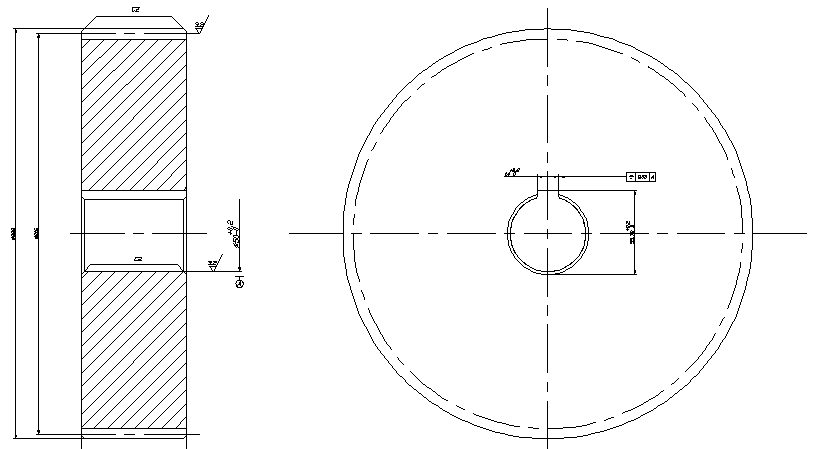
\includegraphics[width=0.5\textwidth]{images/4}
	\end{center}
\end{figure}
\end{frame}

\subsection{蜗轮及蜗杆的选用与校核}

\begin{frame}{蜗轮 蜗杆 类型与材料}
根据GB/T10085-1988的推荐,采用渐开线蜗杆(ZI)

考虑到蜗杆传动功率不大,速度只是中等,故蜗杆用45钢;因希望效率高些,耐磨性好些,故蜗杆蜗杆螺旋齿面要求淬火,硬度为45-55HRC。蜗杆用铸锡磷青铜ZcuSn10P1,金属模铸造。为了节约贵重的有色金属,仅齿圈用青铜制造,而轮芯用灰铸铁HT100制造。
\end{frame}

\begin{frame}{按齿面强度进行设计}
根据闭式蜗杆传动的设计准则,传动中心距:
$$a\geq \sqrt[3]{KT_2\left( \frac{Z_EZ_p}{[\sigma _H]} \right)^2 }$$
\begin{enumerate}[]
	\item 确定作用在蜗杆上的转矩
	
	按$Z_1=2$,估取效率$ \eta =0.75$,则
	$$ T_2=9.55\times 10^6 \frac{P_2}{n_2} =9.55\times 10^6 \frac{p\eta }{n_2/i_{12}}=8247727 N\bullet mm$$
	\item 确定载荷系数
	
	因工作载荷较稳定,故取载荷分布不均匀系数$K_\beta=1$;选取使用系数$K_A=1.15$;由于载荷系数不高,冲击不大,可取动载荷系数$K_v=1.05$;则
	$K=K_A K_\beta K_v=1.21$

\end{enumerate}

\end{frame}


\begin{frame}{按齿面强度进行设计}
	\begin{enumerate}[]
		\item 确定弹性影响系数$Z_E$
		
		因选用的是铸锡磷青铜蜗轮和钢蜗杆相配,故$Z_E=160MP_a^\frac{1}{2}$。
		
		\item 确定接触系数 $Z_p$
		先假设蜗杆分度圆直径$d_1$和传动中心距$a$的比值$\frac{d_1}{a}=0.35$,得$Z_p=2.9$。
		
		
	\end{enumerate}
	
\end{frame}

\begin{frame}{按齿面强度进行设计}
	\begin{enumerate}[]
		
		\item 确定许用接触应力$[\sigma_H]$
		
		根据蜗轮材料为铸锡磷青铜ZcuSnP1,金属模铸造,蜗杆螺旋齿面硬度>45HRC,查得蜗轮的基本许用应力$[\sigma_H]=268MP_a$。
		
		应力循环次数    $N=60jn_2L_h=60\times 1 \times \frac{1980}{60}\times 8 \times 2 \times 250 \times 8 = 6.056\times 10^7$
		
		寿命系数 $K_{HN}=\sqrt[8]{\frac{10^7}{6.056\times 10^7}}=0.99$
		
		则 $[\sigma_H]=K_{HN}\bullet [\sigma_H]'=0.99\times 268 =266MPa$
	
	\end{enumerate}
	
\end{frame}

\begin{frame}{按齿面强度进行设计}
	\begin{enumerate}[]
		
		\item  计算中心距  $$a \geq \sqrt[3] {1.21\times 8247727 \times \left(\frac{160\times 2.9}{260} \right) ^2}=198mm$$
		
		取中心距$a=200mm$,因$i=20$,
		取模数$m=8$,蜗杆分度圆直径$d_1=80mm$。
		这时$\frac{d_1}{a}=\frac{80}{200}=0.4$,
		得接触系数$Z_p'=2.74$,
		因为$Z_p'<Z_p$,因此以上计算结果可用。
	\end{enumerate}
	
\end{frame}


\begin{frame}{蜗杆与蜗轮的主要尺寸与参数}
\begin{enumerate}[]
	\item 蜗杆
	
	轴向齿距$P_a=25.133mm$;\\直径系数$q=10$;\\齿顶圆直径$d_{a1}=96mm$;\\齿根圆直径$d_{f1}=60.8mm$;\\分度圆导程角$\gamma=11\textdegree 18' 36"$;\\蜗杆轴向齿厚$S_a=12.5664mm$。
	
\end{enumerate}
\end{frame}

\begin{frame}{蜗杆与蜗轮的主要尺寸与参数}
	\begin{enumerate}[]
		\item 蜗轮
		
		蜗轮齿数$Z_2=41$;变位系数$x_2=-0.5$;\\
		验算传动比$i=\dfrac{Z_2}{Z_1}=\dfrac{41}{2}=20.5$,这时传动比误差为$\dfrac{20.5-20}{20}=2.5\%$,是允许的。\\
		蜗轮分度圆直径$d_2=mZ_2=8\times 41=328mm$。\\
		蜗轮喉圆直径$d_{a2}=d2+2h_{a2}=344mm$。\\
		蜗轮齿根圆直径$d_{f2}=d_2-2h_{f2}=308.8mm$。\\
		蜗轮咽喉圆半径$r_{g2}=a-\dfrac{1}{2}d_{a2}=28mm$。
		
	\end{enumerate}
\end{frame}


\section{控制部分设计}

\subsection{步进电机的原理}

\begin{frame}{步进电机的原理}
	步进电机是一种能将数字输入脉冲转换成旋转或直线增量运动的电磁执行元件。每输入一个脉冲,电机转轴步进一个步距角增量。电机总的回转角与输入脉冲数成正比例,相应的转速取决于输入脉冲频率。 
\end{frame}

\subsection{步进电机的选择}
\begin{frame}{电机的选择}
	按照工作要求和条件选两相混合式步进电机.
	
	功率
	
	工作所需功率为: $$ P_w = F_w V_w/1000\eta^wkW$$
	$$P_w=T_{nw}/9950\eta^wkW$$
	式中$T=150N\times M$,$\eta_w=36 r/min$ 电机工作效率,$\eta_w=0.97$ 
	$$Pw=150\times 36/(9950\times 0.97 )=3.9kw$$
	电机所需的输出功率为:
	$$P_o=P_w/\eta$$
	
\end{frame}

\begin{frame}{电机的选择}
	
	转矩
	
	由齿轮的转矩可得:$$ T=\dfrac{95.5\times 10^5 p}{n} =1.81 \times 10^4 N\bullet mm$$
	
	确定电机转速
	
	取:
	齿轮传动比:3-5,
	
	蜗杆传动比:15-32,
	
	则总的传动范围为:
	$i=i_1\times i_2 =3\times 15-5*32 =45-160$
	
	电机转速的范围为
	$N=i\times n_m = (45\sim 160)\times 36=1620\sim 5760 r/min$
	为降低电机的重量和价格,选取常用两相混合式步进电机 11BYG250D-0502。
	
\end{frame}

\subsection{步进电机的检验}

\begin{frame}{利用步距角检验}
主要技术参数中,回转精度:$0.03°$、$i=60 $ 可得步距角为: $$\alpha=0.03°\times i=1.8°$$
计算的值与11BYG250D-0502步进电机的步距角相吻合。11BYG250D-0502步进电机满足条件。
\end{frame}

\section{小结}
\begin{frame}{小结}
通过传动方案的设计,机械部分的设计和控制系统的设计,以及相关元件的正确选择和参数的正确计算,本书库转台理论上能够达到所要求的相关功能,在硬件和软件都良好和正常的情况下,此数控分度转台能较好地完成相应的操作。本文设计的数控转台,仅有一个自由度。若在此基础上增加一个或多个自由度,那么工作台的应用范围将会更广,目前市场上多自由度的工作台需求量很大。所以若设计多自由度的数控转台,将会很有价值。
\end{frame}

\begin{frame}[plain]
	
	\begin{center}
		{\LARGE  以上是我对数控转台的设计 }
		\vspace{1cm}
		
		{\LARGE  谢谢大家 }
	\end{center}
	
\end{frame}

\end{document}
